\subsection{Cache Coherence}
In a multi-core system, threads are running concurrently on different cores. These threads may share some
data which they read from or write to. The shared data thus can have multiple copies exist in each core's
private cache. In general, a cache coherence protocol is used to ensure each thread gets the most updated
data to work with.

In a snooping-based protocol, the caches on the same level are connected with a snooping bus. When a request
comes into a cache and incurs a cache miss, a snooping request is sent on the snooping bus. All the other
caches observe the snooping request, and one of them may respond to the request by forwarding the data if 
the data exists. The operations to handle snooping requests and responses highly depend on the specific cache 
coherence protocols being used. Commonly used protocols include MSI, MESI and MOESI~\cite{mark_book}.

% If different timing compartments share data, there is clearly a timing channel introduced by the cache coherence
% protocols. For example, TC0 wants to write to A, and A exists in TC1's cache. In order to perform the write, the
% cache coherence protocol will invalidate A in TC1's cache. Later when TC1 wants to read A, it will incur a cache
% miss which indicates TC0 has written to A. 
In our threat model, timing compartments are allowed to share some OS protected read-only data. This assumption
introduces a timing channel through the cache coherence protocols. Take MOESI protocol as an example, assume TC0 wants
to read a shared data A and incurs a cache miss, while A is in TC1's cache with an Owned(O) state. The MOESI protocol
will forward A to TC0's cache through the snooping bus, which shortens TC0's miss latency compared to accessing the
next level of cache. TC0 then knows A exists in TC1's cache and may correlate this fact with secret information. 
Even if there is no shared data between timing compartments, there still exists a timing channel through the cache
coherence protocol, because the snooping bus is shared by different timing compartments. 
The coherent traffic from different timing compartments can interfere on the snooping bus, thus introduce timing
channels, as demonstrated in the example below.

In this example, we conduct a covert channel attack through cache coherence protocol on a four-core system. 
The system configuration 
is shown in Figure~\ref{fig:coherent_system}. Each core has a private L1 and L2 cache, and the four cores share
the L3 cache. The four L2 caches are connected with a snooping bus which uses a MOESI protocol. 
In this example, there are two attackers who
want to communicate a secret data when the direct communication between them is strictly disallowed. Each attacker 
belongs to a different timing compartment. Attacker0 occupies core 0 and core 1 while attacker1 occupies core 2 and
core 3. 

\begin{figure}
    \begin{center}
        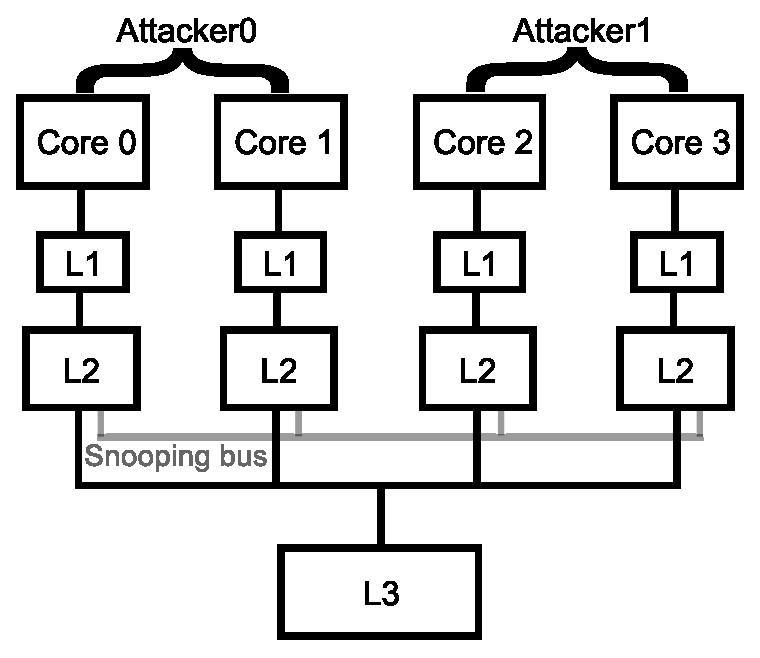
\includegraphics[width=2.3in]{figs/coherent_system.eps}
        \caption{System Configuration}
        \label{fig:coherent_system}
    \end{center}
\end{figure}

Attacker0 has two threads, each running on a different core. Both threads run a $for$ loop of 4000 iterations, and
write to a shared data in each iteration. Before each write is performed, one L2 cache has to forward the data
to the other L2 cache through the snooping bus and invalidates its own copy, according to the cache coherence protocol. 
As a result, there is a lot of coherent traffic between these two threads. Attacker0 runs this $for$ loop repeatedly and
records the time to finish the $for$ loop using c++ timing functions.

Attacker1 owns the secret data ('01101100') and tries to communicate this secret to Attacker0. It checks each bit
in the secret data. If the bit is 0, it executes a $for$ loop which writes to a data in each iteration. This does not produce 
coherent traffic. If the bit is 1, Attacker1 spawns a new thread, which also runs a $for$ loop that writes to the same data, hence producing a lot of coherent traffic. 

\begin{figure}
    \begin{center}
        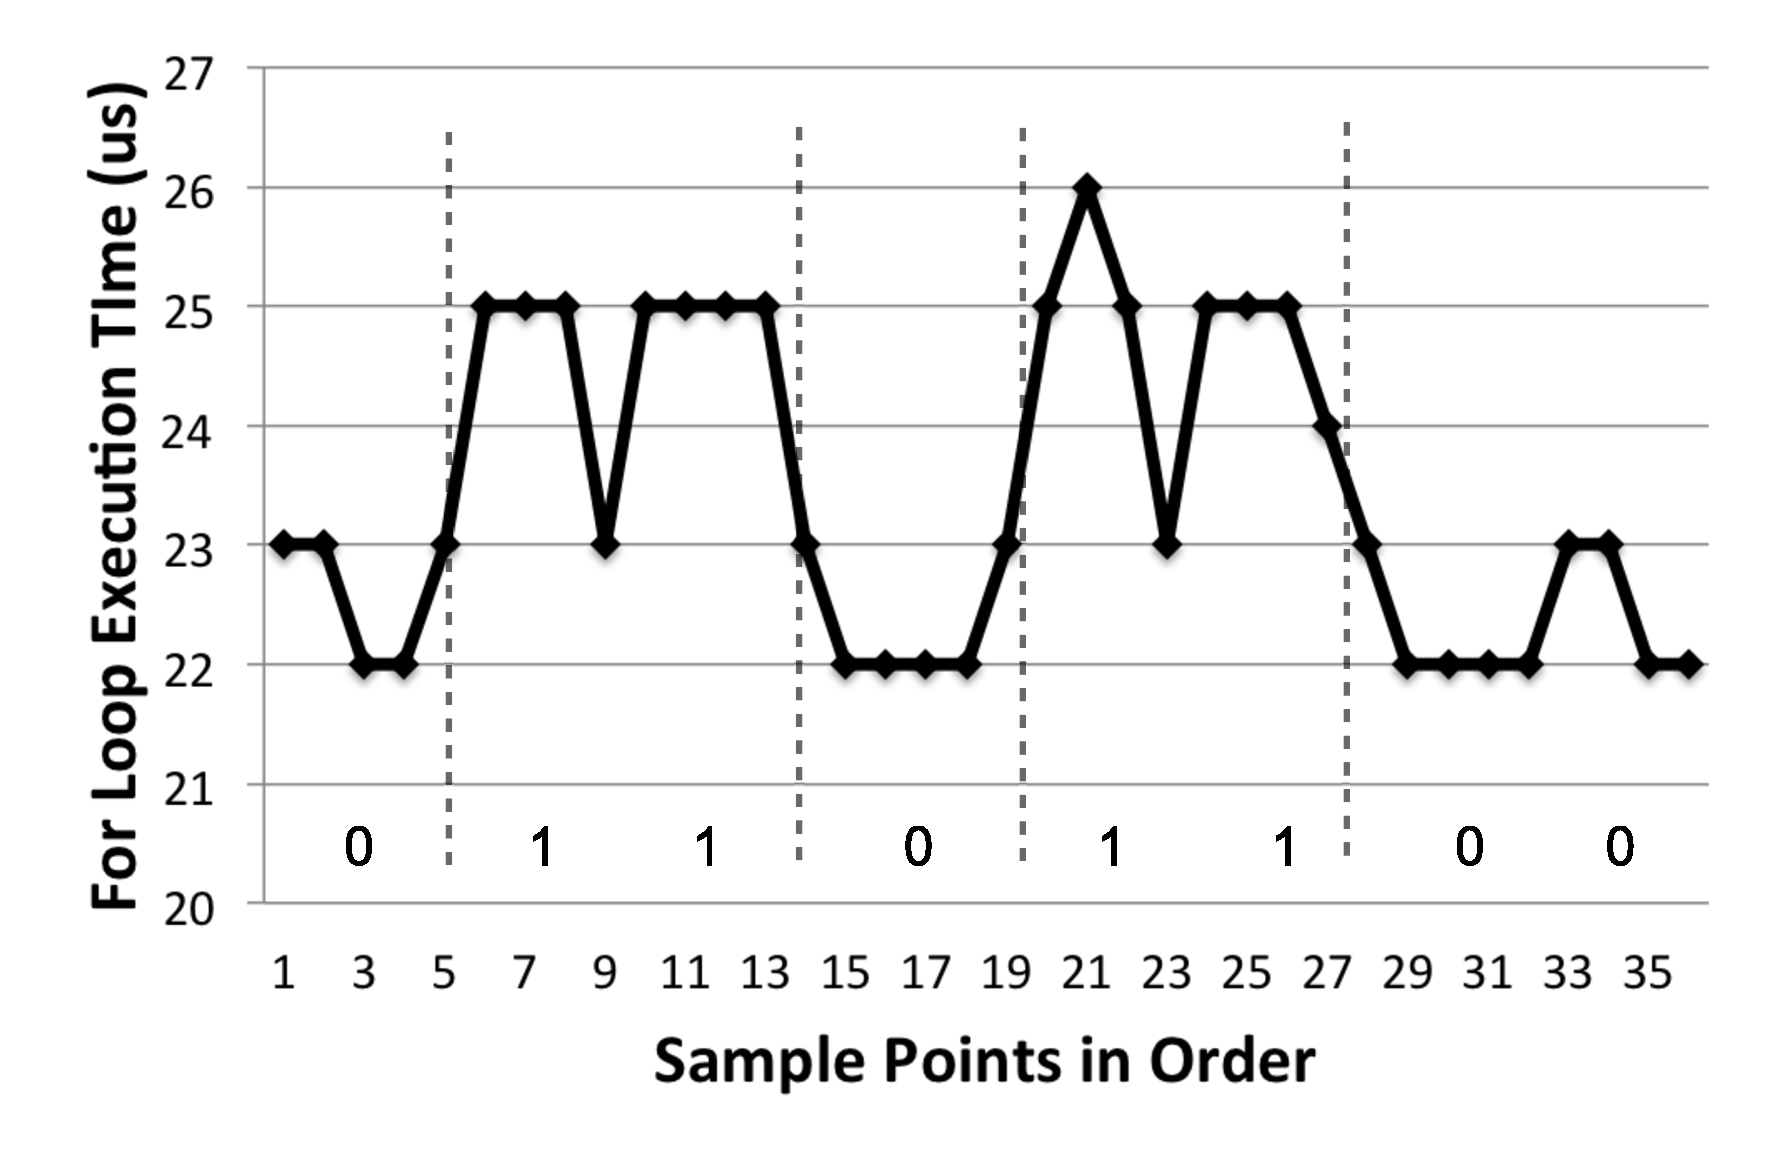
\includegraphics[width=2.79in]{figs/coherence_interference.eps}
        \caption{Attacker0's Timing Observation}
        \label{fig:coherence_interference}
    \end{center}
\end{figure}

Note that in this example, we have all the aforementioned protection schemes implemented except for the snooping bus.
Figure~\ref{fig:coherence_interference} shows the $for$ loop execution time sequence that Attacker0 observes. Each
sample point represents the time it takes to finish a 4000 iteration $for$ loop. Based on the observation, Attacker0
can recover the secret successfully. The timing variation is caused by the interference on the snooping bus. If Attacker1
produces a lot of coherent traffic, Attacker0's coherent traffic gets delayed and thus finishes slower compared to
when Attacker1 does not produce coherent traffic. 

The mechanism to protect against cache coherence timing channels consists of two parts. The first part solves the 
interference on the snooping bus. The snooping bus uses TDM to schedule the snooping requests from different timing
compartments. Each snooping request is attached with a TCID and it can only be sent during its own TC's bus turns.
This protection is the same with what we used for on-chip interconnect. 

The second part deals
with the shared data. Since the shared data is read-only, the cache miss does not necessarily have to be served by
the cache that has the Owned copy. Instead, the cache miss can always be served by the next level of cache or memory.
In our mechanism, when the cache receives a snooping request, it will first check if the TCID of the request matches its
own TCID. If the TCIDs mismatch, then the cache ignores the snooping request even if it has the data, effectively acting
as if the data does not exist. Then the cache miss will be served by the next level of cache. A tricky thing here is
coordinating the operations of multiple level of caches. In some protocols (e.g MOESI), the cache that has the Owned copy
is responsible for responding to the snooping request, so the next level of cache does not respond. In this case, the
cache needs to notify the next level of cache to respond to the snooping request. The notification message should
have a TCID that's the same with the requses so that it does not interfere with its own snooping requests on the snooping 
bus. With our design, the cache that sends a snooping request does not know the data exists on the other cache, while
the timing of the other cache's own operations is not affected.
 

